% ============================================================
% V-B (ext). THỰC NGHIỆM MỞ RỘNG: TÁI CẤU TRÚC KHÔNG GIAN NHÃN
% Nhánh phân tích độc lập — thực hiện SAU khi baseline hoàn tất
% ============================================================
\section{Thực nghiệm mở rộng}

\begin{frame}{Thực nghiệm mở rộng: Mục tiêu và vị trí}
  \begin{alertblock}{Vị trí trong luồng nghiên cứu}
    Baseline đã được train và đánh giá \textbf{hoàn toàn} trên \texttt{FoodSeg103} gốc (103 lớp).
    Nhánh này chạy \emph{sau} và \emph{độc lập} nhằm phân tích bổ sung: liệu phân mảnh nhãn có
    phải một phần nguyên nhân gây lỗi của mô hình nhẹ hay không?
  \end{alertblock}
  \vspace{0.4em}
  \textbf{Câu hỏi nghiên cứu}
  \begin{itemize}
    \item Nếu gộp các lớp ngữ nghĩa gần nhau, mô hình có ổn định hơn không?
    \item Mức độ long-tail có giảm đáng kể sau khi giảm từ 103 xuống 75 lớp?
    \item Kết quả có thể suy ra hướng cải tiến nào cho bài toán gốc không?
  \end{itemize}
  \vspace{0.3em}
  % \begin{block}{Lưu ý}
  %   \texttt{FoodSeg103\_rebalanced} \textbf{không} thay thế đánh giá trên không gian nhãn gốc
  %   và \textbf{không} được dùng làm dữ liệu huấn luyện baseline.
  % \end{block}
\end{frame}

\begin{frame}{Thực nghiệm mở rộng: Phương pháp gộp lớp}
  \begin{columns}[T,onlytextwidth]
    \column[t]{0.59\textwidth}
      \textbf{Tiêu chí gộp (GLCM + quan hệ ngữ nghĩa)}
      \small
      \[
        \mathrm{Sim}(i,j) = \frac{\mathbf{f}_i\cdot\mathbf{f}_j}{\|\mathbf{f}_i\|\|\mathbf{f}_j\|}
      \]
      Hai lớp được gộp khi \textbf{đồng thời} thỏa:
      \begin{itemize}
        \item Gần nhau về mặt ngữ nghĩa (cùng nhóm thực phẩm)
        \item $\mathrm{Sim}(i,j) \geq 0.85$ dựa trên đặc trưng GLCM
      \end{itemize}
      \vspace{0.5em}
      \normalsize
      \textbf{Thống kê trước và sau tái cấu trúc:}

      FoodSeg103 gốc: 103 lớp, 3.982 ảnh train, 2.135 ảnh test.

      Rebalanced: 75 lớp, 3.981 ảnh train, 2.135 ảnh test.
    \column[t]{0.4\textwidth}
      \begin{figure}
        \centering
        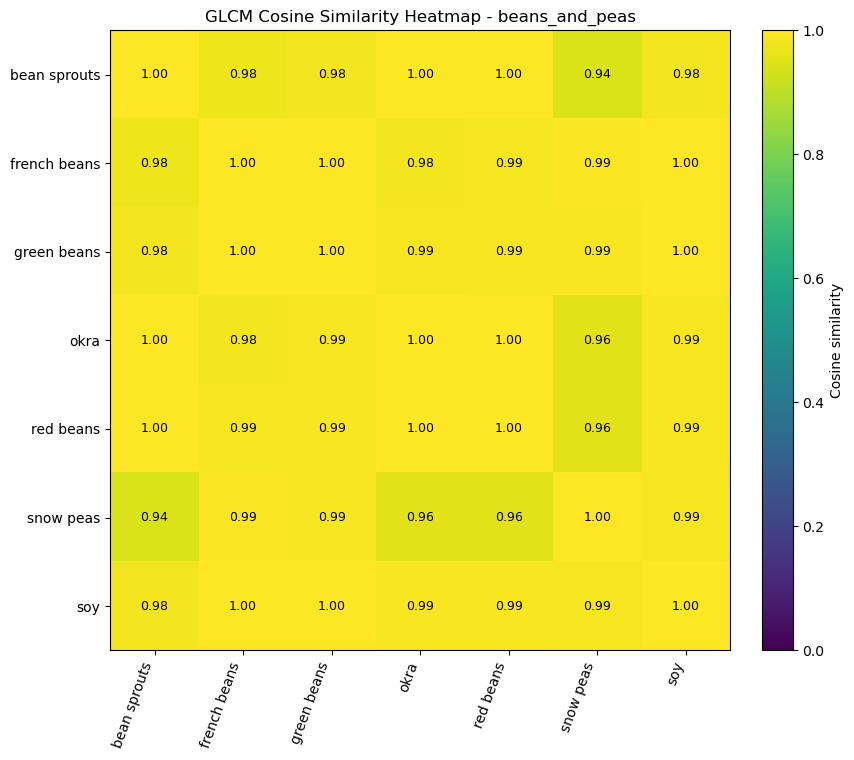
\includegraphics[width=0.85\linewidth]{img/report/analyze/bean_.png}
        \caption{Cosine similarity GLCM (nhóm đậu)}
      \end{figure}
      \begin{figure}
        \centering
        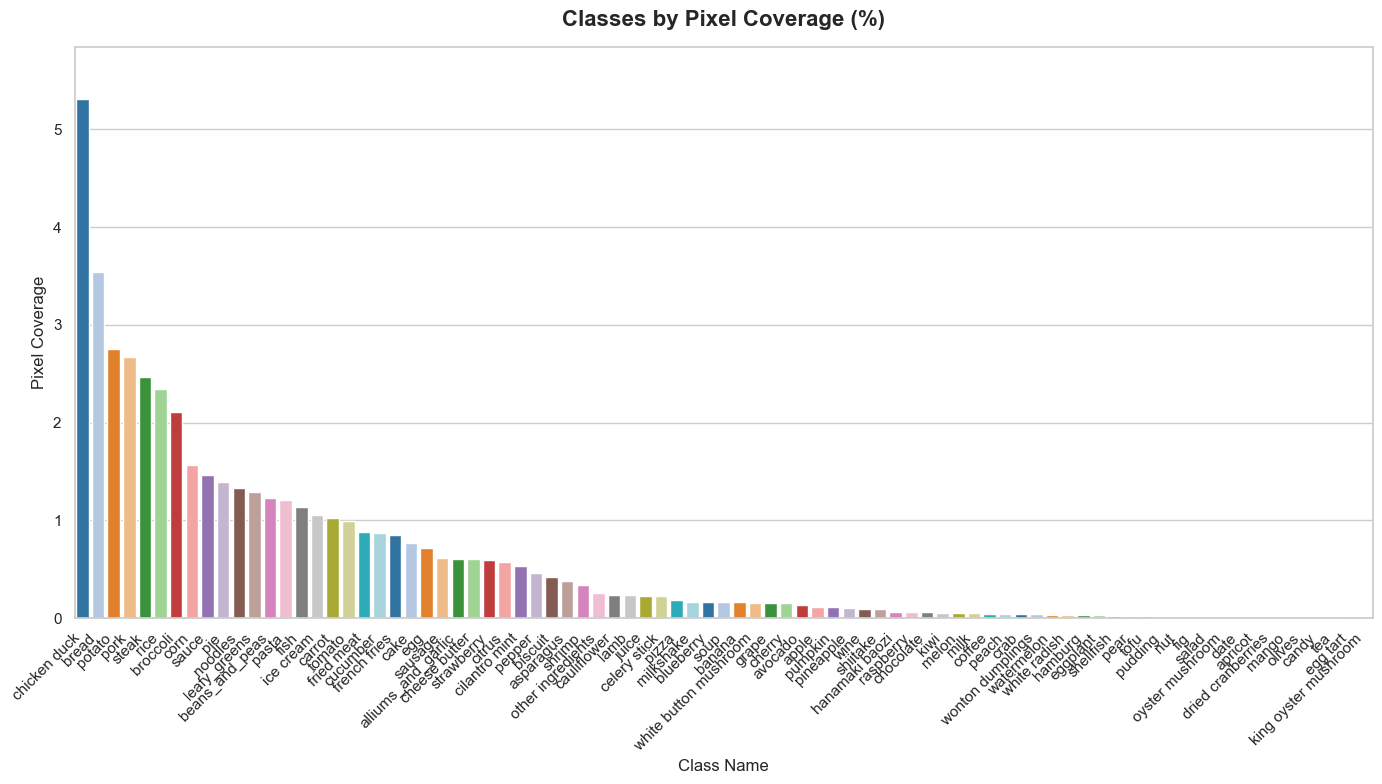
\includegraphics[width=\linewidth]{img/report/analyze/graph_after.png}
        \caption{Phân bố pixel sau tái cấu trúc nhãn}
      \end{figure}
  \end{columns}
\end{frame}

\begin{frame}{Thực nghiệm mở rộng: Kết quả phân tích}
  \begin{block}{Nhận xét chính}
    \begin{itemize}
      \item Giảm phân mảnh nhãn giúp mô hình ổn định hơn ở một số nhóm lớp gần nhau
      \item Long-tail \textbf{chưa biến mất} hoàn toàn sau khi gộp --- 75 lớp vẫn mất cân bằng
      \item Kết quả củng cố nhu cầu xử lý đồng thời: \textbf{texture cục bộ} + \textbf{quan hệ đồng xuất hiện}
    \end{itemize}
  \end{block}
  \vspace{0.4em}
  \begin{alertblock}{Vấn đề cốt lõi vẫn tồn tại}
    Lỗi của BiSeNet trên 103 lớp \textbf{không chỉ} do không gian nhãn quá chi tiết.
    Nguyên nhân cốt lõi vẫn là: texture ambiguity, boundary yếu và sink class ---
    những vấn đề mà 3 module cải tiến đề xuất nhắm trực tiếp vào.
  \end{alertblock}
\end{frame}
